\documentclass [bachelor,german,a4paper,11pt,oneside,webreferences,glossary]{INSOthesis}
% change encoding in the document
\inputencoding{utf8} % default
%\inputencoding{latin1} % for windows

\thesistitle{Evaluierung von REST Frameworks für Android im Kontext des Revex2020 Projekts}
\thesisshorttitle{Evaluierung von REST Frameworks}
%\thesissubtitle{Optional Subtitle} % optional
\thesisdate{\today}

% all titles and designations have to be gender-related!
%\thesistype{Diplomarbeit}{Master's Thesis}
%\thesisdegree{Diplom-Ingenieurin}{Diplom-Ingenieurin}
\thesiscurriculum{Software \& Information Engineering}{Software \& Information Engineering} % your study
\thesisauthor{Elisabeth Pilz} % your name
\thesisauthoraddress{Luegstraße 13, 3340 Waidhofen Ybbs} % your address
\thesismatrikelno{1225231} % your registration number

% advisor
%\thesisauthorpreamble {Verfasser}
%\thesisadvisorpreamble {Betreuung}
%\thesisadvisorone {Thomas Grechenig}
\thesisadvisortwo {Dominik Moser}
%\thesisadvisorthree {Vorname Nachname}

% Bibliographie file
\bibliography{bibliography/references}

\hypersetup{
  %colorlinks=false % enable and disable frames arround links
}

%%%%%%%%%%%%%%%%%%%%%%%%%%%%%%%%%%%%%%%%%%%%%
%
% Can be used to add additional informations
%
%%%%%%%%%%%%%%%%%%%%%%%%%%%%%%%%%%%%%%%%%%%%%
% \AfterTitlePages{}
% \AfterDeclaration{}
% \AfterAcknowledgements{}
% \AfterAbstract{}
% \AfterListOfFigures{}
% \AfterListOfTables{}
% \AfterAbbreviations{}
% \AfterBibliography{}

\renewcommand\afterchapternum{\hspace{1em}}
\begin{document}

\maketitle

%%%%%%%%%%%%%%%%%%%%%%%%%%%%%%%%%%%%%%%%%
%%%   CONTENTS    %%%%%%%%%%%%%%%%%%%%%%%
%%%%%%%%%%%%%%%%%%%%%%%%%%%%%%%%%%%%%%%%%

%%%%%%%%%%%%%%%%%%%%%%%%%%%%%%%%%%%%%%%%%%%%%%%%%%%%%%%%%%%%%%%%%%%%%%%%
\chapter{Einleitung}
\label{sec:introduction}
%%%%%%%%%%%%%%%%%%%%%%%%%%%%%%%%%%%%%%%%%%%%%%%%%%%%%%%%%%%%%%%%%%%%%%%%

%=======================================================================
\section{Problemstellung}
%=======================================================================
Einer der größten Trends auf den Business-Markt ist die Mobilisierung der Geschäftswelt, die sich in den verschiedensten Unternehmensstrategien widerspiegelt. Es gibt zahlreiche Innovationen, um unabhängig von Stakeholdern, Zeit, Ort und Geräten auf Daten und Anwendungen zuzugreifen. Ein wesentlicher Innovationsstrang ist dabei die Entwicklung von Business-Apps, um beispielsweise die Arbeitszeiten auf Geschäftsreisen effektiv ausnützen zu können. Dadurch hat die Bedeutung der Informations- und Kommunikationsindustrie in den letzten Jahren in den Unternehmen stetig zugenommen \cite{smartMobileApps1}.
\\\\
Durch die immer stärkere Nachfrage nach mobilen Apps im Arbeitsalltag ist es notwendig, mobile Endgräte in bestehende Geschäftsprozesse der Unternehmen zu integrieren. Dabei soll es vermieden werden, eine komplett neue IT-Infrastruktur unter Beteiligung von mobilen Endgeräten zu schaffen. In vielen Unternehmen wird daher die IT-Anwendungslandschaft an das Paradigma der serviceorientierten Architektur ausgerichtet. Ein wesentlicher Vorteil dabei ist, dass wohl definierte Schnittstellen vorhanden sind und angebotene Dienste flexibel und plattformunabhängig genutzt werden können. Sollen nur mobile Anwendungen in die existierende IT-Anwendungslandschaft eingegliedert werden, bedeutet dies in der serviceorientierten Architektur, das Web Services benötigt werden. In der Praxis werden Web Services entweder mit dem Kommunikationsprotokoll \acrfull{SOAP} oder \acrfull{REST} umgesetzt \cite{smartMobileApps17}.
\\\\
Im Revex2020 Projekt wird das Kommunikationsprotokoll REST verwendet, dadurch ist es nötig ein geeignetes Framework aufseiten der mobilen App zu finden, dass eine vollständige und korrekte Anbindung an den Webservice ermöglicht. Es existieren bereits zahlreiche Frameworks, die eine REST Implementierung unterstützen, diese unterscheiden sich aber stark in der Qualität und im Funktionsumfang. Auch bieten nicht alle diese Frameworks eine Unterstützung für Android an. Daher ist die Auswahl eines geeigneten Frameworks für eine erfolgreiche Implementierung ausschlaggebend. 

%=======================================================================
\section{Motivation}
%=======================================================================

Die Thematik rund um REST-Frameworks für Android ist noch relativ neu, dadurch ist es nicht möglich ohne größere Recherchen ein geeignetes Framework für das Projekt Revex2020 auszuwählen. Es gibt zwar einige Vergleiche von REST Frameworks, wie etwa die Fachstudie von Markus Fischer, Kalman Kepes und Alexander Wassiljew \cite{vergleich13}. In dieser Studie wird allerdings nicht darauf eingegangen, ob die Frameworks eine Implementierung clientseitig mit Android unterstützen, es wird die vermehrt auf die serverseitige Implementierung eingegangen. Die Möglichkeit der clientseitigen Implementierung ist aber eine essenzielle Anforderung, da eine Business-App für Android entwickelt werden soll. 
\\\\
Der immer stärker wachsende Bereich von mobilen Anwendungen macht das zu untersuchende Thema besonders interessant. Herkömmliche Software rückt immer weiter in den Hintergrund, Daten sollen sofort und überall abgerufen werden können. Mobile Endgeräte wie Smartphone und Tablets verändern daher die Geschäftswelt nachhaltig, Führungskräfte und Mitarbeiter erhalten jederzeit Zugang zu Unternehmensinformationen und -prozessen. Die Unternehmen der Zukunft werden daher mobil \cite{smartMobileApps7}.  
\\\\
Revex2020 ist ein Forschungsprojekt zur Revitalisierung von Wasserkraftwerken, das in Kooperation mit dem Institut für Energietechnik und Thermodynamik entwickelt wird \cite{doujak}. Ein Ziel dieses Projektes ist es, Mitarbeitern zukünftig zu ermöglichen, mithilfe von mobilen Endgeräten den Zustand einzelner Kraftwerkskomponenten vor Ort erfassen zu können. Es soll eine Android-App entwickelt werden, die das bereits vorhandene Backend, über das REST-Webservices nutzt um exemplarisch den Anwendungsfall abzubilden.

%=======================================================================
\section{Zielsetzung}
%=======================================================================

Ziel dieser Bachelorarbeit ist die Evaluierung verschiedener REST-Frameworks für Android im Kontext des Revex2020 Projekts, um eine unkomplizierte Anbindung an das bereits vorhandene Backend zu ermöglichen. Dazu werden bestehende REST-Frameworks für Android getestet, indem diese in einem Anwendungsfall eingesetzt werden. Nach der Evaluierung dieser Frameworks soll eine Empfehlung abgegeben werden, welches sich am besten für das Revex2020 Projekt eignet.
\\\\
Die Evaluierung der Frameworks erfolgt anhand von Prototypen, indem die REST-Frameworks verwendet werden. Es wurden im Vorfeld verschiedene Anwendungsfälle definiert (siehe Abbildung \ref{figure:useCase}), indem die einzelnen REST Frameworks integriert werden. Dabei werden in einem Szenario verschiedene Prozesse durchgespielt, wie Kraftwerk erstellen, löschen, bearbeiten und anzeigen. Als Vorlage dazu wurde die bestehende Web-Applikation des Projektes verwendet.
\\\\

\begin{minipage}{\textwidth} 
	\centering	
	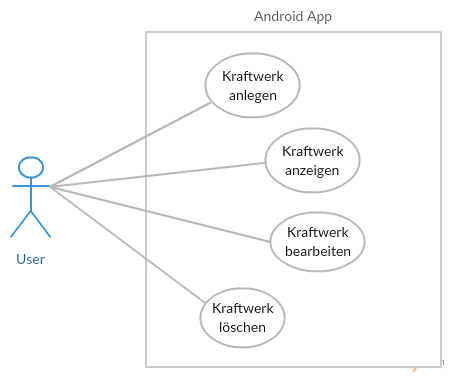
\includegraphics[width=0.65\textwidth]{figures/kraftwerke_use_case.png}
	\captionof{figure}{Use-Case-Diagramm}
	\label{figure:useCase}
	\vspace{2ex}
\end{minipage}

%=======================================================================
\section{Methodik}
\label{sec:methodik}
%=======================================================================
Die Qualität der einzelnen Frameworks soll anhand folgender Kriterien verglichen werden, welche an dem Kriterienkatalog der Fachstudie "Vergleich von Frameworks zur Implementierung von REST-basierten Anwendungen" \cite{vergleich13} angelehnt sind. Dieser Kriterienkatalog beschäftigt sich mit den Eigenschaften für die Evaluierung von REST Frameworks, vor allem auf serverseitiger Sicht. Der Kriterienkatalog wurde deshalb gekürzt bzw. einzelne Punkte zusammengefasst und abgeändert, um eine Evaluierung im Kontext des Projektes Revex2020 durchführen zu können. 
\\\\
Das Hauptaugenmerk der Evaluierung liegt auf der Clientseite, da die entwickelte App eine Client Applikation darstellt. Deswegen wurden spezifische Kriterien der Fachstudie zu einer REST Server Applikation gestrichen. Beispielsweise wurde der gesamte Kriterienblock über Ressourcentypen \cite{ressourcen:rest} weggelassen, da es für die clientseitige Verarbeitung irrelevant ist, welche Ressourcentypen serverseitig implementiert werden können. 
\\\\
\textbf{Entwicklungskultur rund um die Frameworks:}
\begin{itemize}
	\item Unter welcher Lizenz steht das Projekt zur Verfügung?
	\item Existiert eine aktive Community?
	\item Ist eine Dokumentation des Codes vorhanden? (Schnittstellenbeschreibung, JavaDoc)	
	\item Gibt es Hilfestellung für Entwicklung? (Tutorial, Codebeispiele)
\end{itemize}

\textbf{Implementierung der REST-Frameworks:}
\begin{itemize}
	\item Wie aufwendig ist es das Framework ins Projekt einzubinden? 
	\item Welche HTTP-Methoden werden unterstützt? (GET, POST, PUT, DELETE etc.)
	\item Gibt es Möglichkeiten den HTTP-Header zu verändern oder zu erweitern?
	\item Welche Medientypen werden unterstützt? (JSON, HTML, XML etc.)
	\item Kann die URL zum Abfragen von Resourcen dynamisch verändert werden? (z.B. über Parameter steuern)
	\item Gibt es eine Möglichkeit für asynchronen Nachrichtenaustausch?
	\item Wird das HATEOAS-Konzept* unterstützt?
	\item Wird ein Error-Handling unterstützt?	
\end{itemize}

\textbf{Performance und benötige Speicherplatz der Frameworks:}
\begin{itemize}
	\item Wie stark wird die CPU belastet?  
	\item Wie viel RAM wird benötigt? 
	\item Wie schnell erfolgt die Abwicklung einzelner Requests (GET, POST)?
	\item Wie groß ist die erzeugte .apk-Datei?	
\end{itemize}
\newpage
\textbf{Erweiterte Technische Fähigkeiten der Frameworks:}
\begin{itemize}
	\item Wie wird Sicherheit gehandhabt?  (Authentifizierung)
	\item Werden andere Protokolle fernab von HTTP unterstützt?	
	\item Unterstützt das Framework die Entwicklung von Server Applikationen?
	\item Bietet das Framework zusätzliche Dienst fernab der REST-Kommunikation an?
	\item Wird transaktionales Verhalten vom Framework unterstützt? (ACID**-Eigenschaften)\\
\end{itemize}

* Das \textbf{HATEOAS}-Konzept wird in Kapitel \ref{sec:rest} genauer beschrieben.
\\\\
** \textbf{ACID} seht für Atomicity, Consistency, Isolation und Durability. Dieses Konzept beschreibt, dass alle Daten die während einer Transaktion verwendet werden, gesperrt sind und sich nicht ändern dürfen, so lange bis die Transaktion Commited wird oder ein Rollback durchgeführt wird. Das Einhalten dieser Eigenschaften ist wichtig, da die Kommunikation zu Servern über zustandslose REST-Schnittstellen abgewickelt wird. Durch die Zustandslosigkeit der Anfragen kann es bei Fehlern schnell zu einer Dateninkonsistenz auf dem Server kommen \cite{braun:Transaktionen}.

%%%%%%%%%%%%%%%%%%%%%%%%%%%%%%%%%%%%%%%%%%%%%%%%%%%%%%%%%%%%%%%%%%%%%%%%
\chapter{State of the Art}
\label{sec:stateOfTheArt}
%%%%%%%%%%%%%%%%%%%%%%%%%%%%%%%%%%%%%%%%%%%%%%%%%%%%%%%%%%%%%%%%%%%%%%%%

Um Rest Frameworks für die Evaluierung zu finden, wurde eine Technologierecherche durchgeführt. Dabei konnten folgende Projekte gefunden werden, welche eine REST-Anbindung für Android unterstützen:
\begin{itemize}
	\item Resty (\href{http://beders.github.io/Resty/Resty/Overview.html}{http://beders.github.io/Resty/Resty/Overview.html})
	\item Retrofit (\href{http://square.github.io/retrofit/}{http://square.github.io/retrofit/})
	\item RESTlet (\href{http://restlet.com/}{http://restlet.com/})
	\item Spring for Android (\href{http://projects.spring.io/spring-android/}{http://projects.spring.io/spring-android/})
	\item CRest (\href{http://crest.codegist.org/index.html}{http://crest.codegist.org/index.html})
	\item RESTeasy Mobile (\href{http://resteasy.jboss.org/}{http://resteasy.jboss.org/})
	\item RESTDroid (\href{http://pcreations.fr/me/restdroid-resource-oriented-rest-client-for-android}{http://pcreations.fr/me/restdroid-resource-oriented-rest-client-for-android})
	\item Jersey (\href{https://jersey.java.net/}{https://jersey.java.net/})
\end{itemize}

Es würde den Rahmen der Bachelorarbeit überschreiten, all diese gefundenen REST Frameworks zu evaluieren. Es wurde daher einer Vorstudie gemacht, aufgrund derer die Drei populärsten und den Anforderungen adäquatesten Frameworks ausgewählt wurden.
\\\\
Die Popularität eines Frameworks gibt eine gewisse Auskunft über die Qualität, da für diese Frameworks oft besserer Support in Form von Dokumentation zur Verfügung steht. Eine Studie von Chris Parnin\cite{parnin2012crowd} beschäftigen sich damit, wie "'Crowd documentation"' beispielsweise auf Question and Answer (Q\&A) Webseiten, die Hilfestellung zu verschiedenen Frameworks beeinflusst. Verwenden viele Entwickler ein Framework, sind dadurch mehr Fragen auf Q\&A Webseiten vorhanden und dadurch können mögliche Fragen besser beantwortet werden. Durch eine Erhebung der Anzahl von Fragen auf Stack Overflow\footnote{\href{http://stackoverflow.com/}{http://stackoverflow.com/}} und der Stars auf GitHub\footnote{\href{https://github.com/}{https://github.com/}} wurden Rückschlüsse auf die Popularität der einzelnen Frameworks gezogen.  
\\\\
In dem Artikel "'How to identify a strong open source project"\cite{balter:strongOS} werden verschiedene Indikatoren erhoben, welche Rückschlüsse auf eine solide und gute Entwicklung eines Frameworks geben. Deswegen wurden zusätzlich noch verschiedene Aktivitäten auf GitHub verglichen, wie Datum des letzten Commits oder Anzahl der Commits.

\begin{minipage}{\textwidth} 
	\centering	
	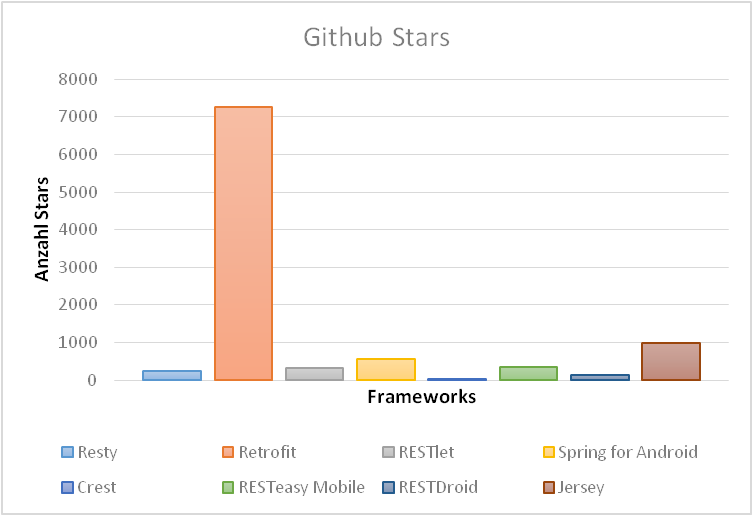
\includegraphics[width=0.65\textwidth]{figures/github_stars.png}
	\captionof{figure}{Github Stars, abgerufen am 25.09.2015}
	\label{figure:githubStars}
	\vspace{2ex}
\end{minipage}

\begin{minipage}{\textwidth} 
	\centering	
	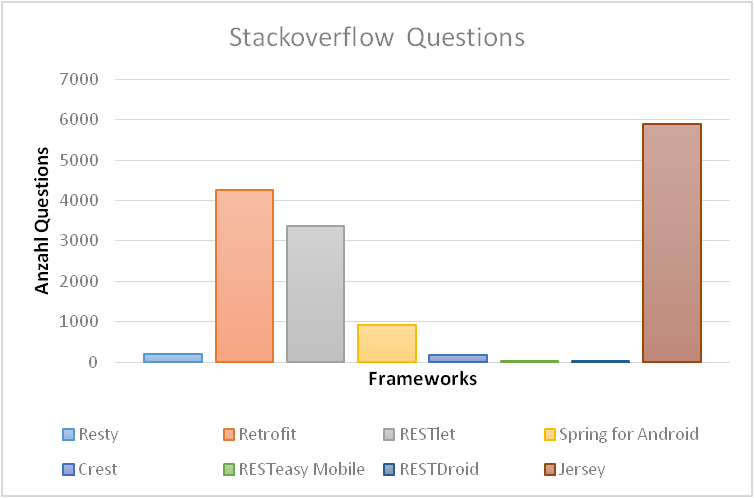
\includegraphics[width=0.65\textwidth]{figures/stackoverflow_questions.png}
	\captionof{figure}{Stackoverflow Questions, abgerufen am 24.09.2015}	
	\label{figure:stackoverflowQuestions}
	\vspace{2ex}
\end{minipage}

\begin{minipage}{\textwidth} 
	\centering	
	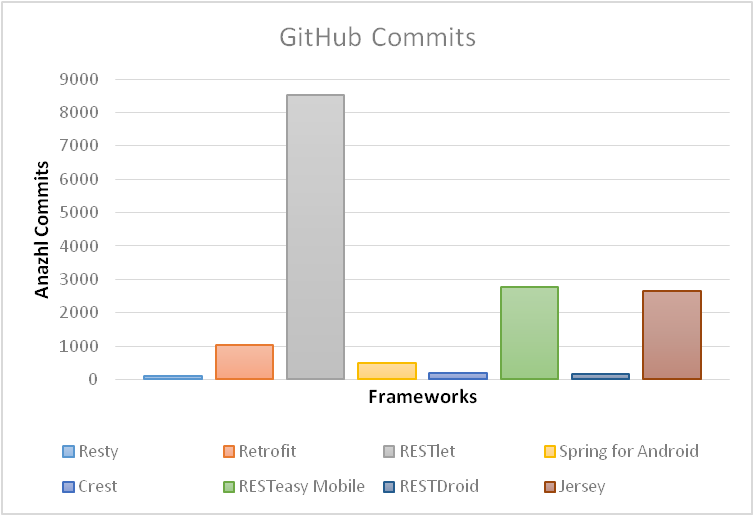
\includegraphics[width=0.65\textwidth]{figures/github_commits.png}
	\captionof{figure}{Github Commits, abgerufen am 25.09.2015}	
	\label{figure:githubCommits}
	\vspace{2ex}
\end{minipage}

\begin{minipage}{\textwidth} 
	\centering	
	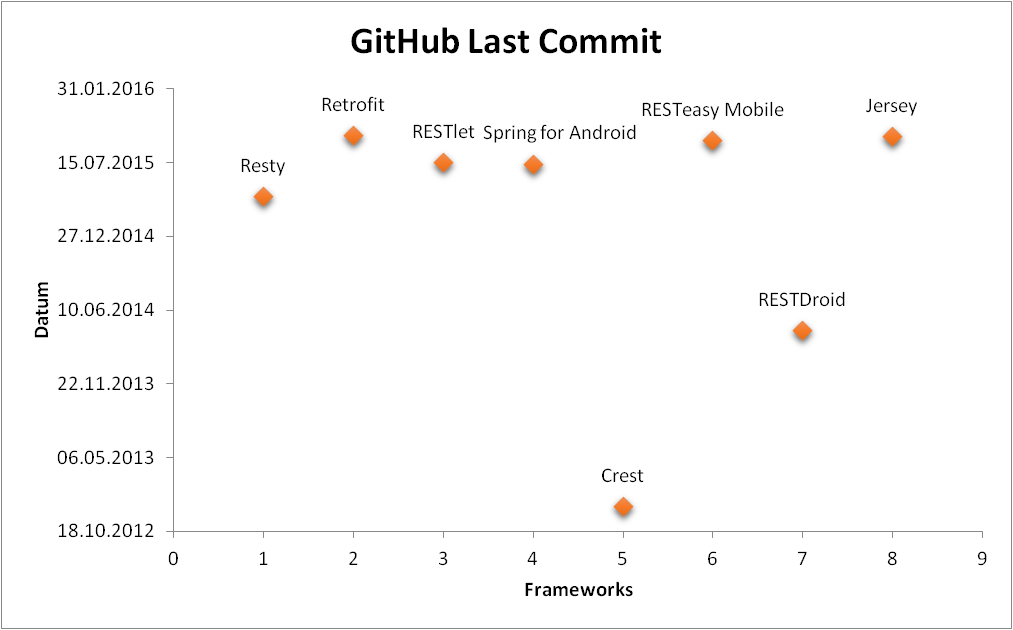
\includegraphics[width=0.65\textwidth]{figures/github_lastCommit.png}
	\captionof{figure}{GitHub Last Commit, abgerufen am 28.09.2015}	
	\label{figure:githubLastCommit}
	\vspace{5ex}
\end{minipage}

Aufgrund der Vorstudie werden folgende REST-Frameworks evaluiert und miteinander verglichen:

\begin{itemize}
	\item Retrofit 
	\item Jersey
	\item Spring for Android
\end{itemize}

% insert bibliography and such stuff
\BackMatter

\cleardoublepage
\appendix

%%%%%%%%%%%%%%%%%%%%%%%%%%%%%%%%%%%%%%%%%%%%%%%%%%%%%%%%%%%%%%%%%%%%%%%%
\chapter{\appendixlabel}
%%%%%%%%%%%%%%%%%%%%%%%%%%%%%%%%%%%%%%%%%%%%%%%%%%%%%%%%%%%%%%%%%%%%%%%%



\end{document}
